\begin{figure}
    \centering
    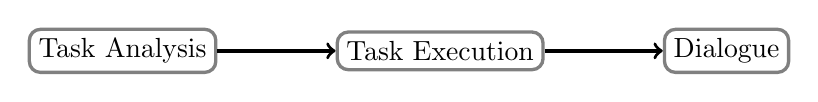
\begin{tikzpicture}
        \node[right] at (0, 0) (task)[rectangle, rounded corners, text centered, draw=gray, very thick] {Task Analysis};
        \draw [very thick, ->] (task.east) -- ++(1.5cm, 0) 
            node[right] (exec)[rectangle, rounded corners, text centered, draw=gray] {Task Execution};
        \draw [very thick, ->] (exec.east) -- ++(1.5cm, 0)
            node[right] (dial)[rectangle, rounded corners, text centered, draw=gray] {Dialogue};
        \end{tikzpicture}
    \caption{Model to identify peer interactions between participants}
    \label{fig:peer-model}
\end{figure}
